% Track 1 — methods report. Compile: latexmk -lualatex track1.tex (see scripts/compila_informes.py)
\documentclass[10pt]{article}
\usepackage{mvareport}
\renewcommand{\reporttrack}{TRACK 1 · VARIANT PREDICTION}
\renewcommand{\reportshort}{Biallelic \textit{BUB1B} in MVA}
\hypersetup{pdftitle={Track 1 methods report: biallelic BUB1B in mosaic variegated aneuploidy},pdfauthor={Agustín Pérez Castro (aperezcastro)}}

\defref{hanks}{Hanks et al.}{2004}\defref{suij}{Suijkerbuijk et al.}{2010}\defref{sieben}{Sieben et al.}{2020}
\defref{spliceai}{Jaganathan et al.}{2019}\defref{exomiser}{Smedley et al.}{2015}\defref{richards}{Richards et al.}{2015}
\defref{pvs1}{Abou Tayoun et al.}{2018}\defref{tavtigian}{Tavtigian et al.}{2020}\defref{alphamissense}{Cheng et al.}{2023}
\defref{matsuura}{Matsuura et al.}{2006}\defref{bohers}{Bohers et al.}{2008}\defref{nishitani}{Nishitani-Isa et al.}{2019}
\defref{nakano}{Nakano et al.}{2024}\defref{baker04}{Baker et al.}{2004}\defref{malumbres}{Malumbres}{2024}
\defref{snape}{Snape et al.}{2011}\defref{yost}{Yost et al.}{2017}

\begin{document}

\reportheader{Rare Disease, Real Kid · MVA Hackathon 2026 · Track 1 methods report}
{Biallelic \textit{BUB1B} in a child with mosaic variegated aneuploidy}
{Three independent analysis arms converge on a null + hypomorphic allele pair (MVA type 1)}
{Agustín Pérez Castro (\texttt{aperezcastro}, individual)\enspace·\enspace Proband PROBAND01\enspace·\enspace October 2026\\
Code: \href{https://github.com/aperezcastro/hackaton-genetico}{github.com/aperezcastro/hackaton-genetico} (CC BY 4.0)}
{This report shows only the submitted candidate variants and aggregate statistics. No genome-scale table, read or
genotype list leaves the protected compute environment (§\ref{sec:data}).}

\begin{keybox}[title={Answer at a glance}]
\begin{tabularx}{\linewidth}{@{}P{3.1cm}L@{}}
\sffamily\small\bfseries Gene & \sffamily\small \gene{BUB1B} (15q15.1; NM\_001211.6 / ENST00000287598.11, MANE Select), compound heterozygous, phase inferred \\
\sffamily\small\bfseries Allele 1 · null & \sffamily\small chr15:40209701 T>G · c.2210T>G · p.(Leu737*) · stop-gained, exon 17/23, NMD predicted · ClinVar P/LP · \textbf{Likely pathogenic (9 points), Pathogenic with ClinVar corroboration} \\
\sffamily\small\bfseries Allele 2 · hypomorph & \sffamily\small chr15:40220612 T>G · c.3006T>G · p.(Asn1002Lys) · kinase-domain missense, last exon · ultra-rare · AlphaMissense 0.92 · \textbf{VUS (4--5 points)} \\
\sffamily\small\bfseries Disease & \sffamily\small MVA type 1 (OMIM \#257300), autosomal recessive \\
\sffamily\small\bfseries Independent check & \sffamily\small Exomiser 15.1 ranks \gene{BUB1B} first genome-wide, with and without a phenotype pre-filter \\
\sffamily\small\bfseries Submission & \sffamily\small 3 rows: the pair (EPCR 0.95) + two low-probability pairings with a third, deep-intronic \gene{BUB1B} variant (0.03, 0.01)
\end{tabularx}
\end{keybox}

\vspace{2pt}
\noindent\statnum{4.96\,M}{normalised variants in the VCF}\hfill
\statnum{1}{gene left by the unbiased funnel and the panel}\hfill
\statnum{\#1}{\gene{BUB1B} rank in Exomiser (of $\sim$20,000 genes)}\hfill
\statnum{0}{runs of homozygosity > 2 Mb (no autozygosity)}

\section{Summary}

The genotype reproduces the textbook molecular architecture of MVA1. One allele is truncating (transcript degraded by
NMD; no protein expected), and the other is a missense allele in the C-terminal kinase domain, where most MVA1 missense alleles act by lowering BUBR1
abundance \citep{hanks,suij}. Whether this particular allele lowers abundance or impairs function has not been
measured; the Track~2 report carries both scenarios. The pair is
architecturally analogous to the alleles modelled in mice by \citet{sieben}: BubR1 X753 (truncating) + L1002P (kinase-domain
missense; mouse L1002 = human L1012). Our alleles are p.Leu737* and p.Asn1002Lys. That mouse genotype died
prematurely, while the child is alive, which suggests the child's missense allele keeps more function.

Five design choices shaped the analysis:
\begin{enumerate}[label=(\roman*)]
\item a \textbf{three-arm strategy} (Figure~\ref{fig:overview}): an unbiased genome-wide search run in parallel with a
  hypothesis-driven MVA/spindle-assembly-checkpoint (SAC) panel and a phenotype-driven ranking, so that the answer is not just ``where we looked'';
\item because the second, hypomorphic MVA1 allele is often subtle, the panel was searched at \textbf{every
  consequence class} and scored for splicing;
\item \textbf{explicit, calibrated evidence}: ACMG/AMP criteria with Bayesian points for every submitted variant;
\item \textbf{genome-level checks from aggregate statistics}: allelic balance, mosaicism and autozygosity;
\item \textbf{data protection by design}: patient data stayed in a private cloud environment, with no third-party
  variant APIs.
\end{enumerate}

\begin{figure}[htbp]
\centering
\begin{tikzpicture}[font=\sffamily\scriptsize, node distance=4mm and 5mm,
  box/.style={draw=rule, fill=white, rounded corners=2pt, align=center, inner sep=3.5pt, minimum height=8mm, text width=#1},
  box/.default=2.5cm, flow/.style={-{Stealth[length=2mm]}, draw=ink2, line width=0.6pt}]
  \node[box=2.1cm, fill=panel] (vcf) {\textbf{Proband VCF}\\4.96\,M variants};
  \node[box=2.4cm, right=of vcf] (ann) {\textbf{Normalise + annotate}\\bcftools · VEP 116\\gnomAD v4.1 · ClinVar\\AlphaMissense};
  \node[box=2.9cm, right=10mm of ann, yshift=11mm, draw=brand, line width=0.7pt] (arm1) {\textbf{Arm 1 · unbiased}\\genome-wide funnel +\\recessive gene model};
  \node[box=2.9cm, below=3.5mm of arm1, draw=violet, line width=0.7pt] (arm2) {\textbf{Arm 2 · hypothesis}\\MVA/SAC panel, every\\consequence + SpliceAI};
  \node[box=2.9cm, below=3.5mm of arm2, draw=aqua, line width=0.7pt] (exo) {\textbf{Arm 3 · phenotype}\\Exomiser 15.1, 8 HPO\\terms, ± pre-filter};
  \node[box=2.6cm, right=10mm of arm2, fill=panel] (int) {\textbf{Integration}\\ACMG/AMP + Bayesian\\points · phase test\\genome-level QC};
  \node[box=1.9cm, right=of int, fill=brand!12, draw=brand] (out) {\textbf{Ranked CSV}\\3 rows · EPCR};
  \node[box=2.1cm, below=4mm of vcf, fill=white, draw=muted, dashed] (hpo) {\textbf{Clinical summary}\\8 HPO terms (IDs only)};
  \draw[flow] (vcf) -- (ann);
  \draw[flow] (ann.east) -- ++(4mm,0) |- (arm1.west);
  \draw[flow] (ann.east) -- ++(4mm,0) |- (arm2.west);
  \draw[flow] (ann.east) -- ++(4mm,0) |- (exo.west);
  \draw[flow] (hpo.east) -- (exo.west -| ann.east) -- (exo.west);
  \draw[flow] (arm1.east) -- ++(4mm,0) |- (int.west);
  \draw[flow] (arm2.east) -- (int.west);
  \draw[flow] (exo.east) -- ++(4mm,0) |- (int.west);
  \draw[flow] (int) -- (out);
\end{tikzpicture}
\caption{Analysis overview. Three arms (unbiased, hypothesis-driven, phenotype-driven) were run independently and
only then integrated; all converge on the same \gene{BUB1B} pair. Heavy steps run as time- and cost-capped jobs on
Modal (total compute for Track~1 $\approx$ 1.4~USD, logged in \code{scripts/modal/gastos.csv}).}
\label{fig:overview}
\end{figure}

\section{Data and reference}

\begin{itemize}
\item \textbf{Input:} single-sample WGS VCF from the organisers (Sentieon 202308.02 + GATK VariantFiltration), GRCh38
  no-alt analysis set + hs38d1 decoys, contigs without the \code{chr} prefix. No parental data, no BAM/CRAM.
\item \textbf{Phenotype:} 8 HPO terms extracted from the clinical summary as IDs only and resolved locally against
  \code{hp.obo}: rhabdomyosarcoma (HP:0002859), nephrocalcinosis (HP:0000121), short stature (HP:0004322), failure to
  thrive (HP:0001508), skeletal muscle atrophy (HP:0003202), premature birth (HP:0001622), small for gestational age
  (HP:0001518), recurrent spontaneous abortion (HP:0200067, family history).
\item \textbf{Coordinates:} GRCh38, 1-based, VCF-normalised (left-aligned, parsimonious), with the \code{chr} prefix
  required by the submission format.
\end{itemize}

\begin{table}[H]
\tablefont
\begin{tabularx}{\linewidth}{@{}P{2.7cm}LP{2.75cm}@{}}
\toprule
\thead{Step} & \thead{Tool / version} & \thead{Script} \\
\midrule
Normalisation & bcftools norm \code{-m -any}, left-alignment against the Ensembl GRCh38 primary assembly & \code{anotar.py} \\
Annotation & Ensembl VEP 116 offline (\code{--everything}, MANE, HGVS); gnomAD v4.1 exomes + genomes; ClinVar (cache + NCBI VCF with review status); SIFT, PolyPhen-2, AlphaMissense (hg38) & \code{anotar.py} \\
Funnel + panel & Python, per chromosome on Modal & \code{filtra.py} \\
Splicing & SpliceAI 1.3.1, GENCODE grch38 annotation, windows of 50 and 2,000 nt & \code{splice\_ai.py} \\
Phenotype ranking & Exomiser 15.1.0, data release 2512 (hg38, phenotype), hiPHIVE, REVEL/MVP/AlphaMissense/SpliceAI & \code{exomiser.py} \\
Phase feasibility & heterozygous-site spacing in the inter-allele interval & \code{fase\_viable.py} \\
Genome-level QC & allelic balance per chromosome and in 5-Mb bins; runs of homozygosity & \code{balance\_alelico.py} \\
Validation & organisers' \code{evaluation.py} & — \\
\bottomrule
\end{tabularx}
\caption{Pipeline components (in \code{scripts/modal/}; the structural context of Figure~\ref{fig:proteina} comes from
\code{scripts/t2/estructura.py}). \code{evaluation.py} is the organisers' public scorer from the hackathon Space.}
\end{table}

\section{Arm 1 — unbiased genome-wide funnel}

\begin{figure}[htbp]
\centering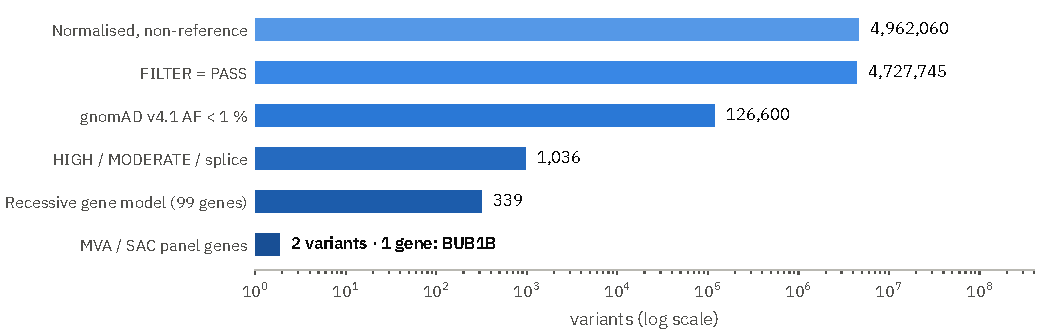
\includegraphics[width=\linewidth]{fig/t1_embudo.pdf}
\caption{Variant funnel. Each step is a single, stated criterion. The recessive gene model keeps genes with
$\geq$2 heterozygous or 1 homozygous qualifying variants; of its 99 genes only \gene{BUB1B} belongs to the MVA/SAC
panel. The other 98 genes were reviewed one by one (§\ref{sec:alt}).}
\label{fig:embudo}
\end{figure}

\textit{Thresholds.} AF < 1\,\% is deliberately permissive for a recessive disease with fewer than 50 known patients.
The maximum credible population AF of a pathogenic recessive allele is far lower, but a loose cut avoids discarding
hypomorphic alleles that may be enriched in a founder population. 65,992 variants remain at AF < 0.1\,\%.

\section{Arms 2 and 3 — the MVA/SAC panel and the phenotype}

\textbf{Panel} (\code{filtra.py}): established MVA genes \citep{malumbres} \gene{BUB1B} (MVA1), \gene{CEP57} (MVA2;
\citealp{snape}), \gene{TRIP13} (MVA3; \citealp{yost}) and \gene{CENATAC/CCDC84} (MVA4); SAC and kinetochore genes (\gene{BUB1, BUB3, MAD1L1, MAD2L1, MAD2L1BP, TTK,
KNL1, ZW10, KNTC1, SPC24/25, CENPE, INCENP, BIRC5, SGO1}…); cohesion and SMC5/6 genes (\gene{SMC5, SMC6, NSMCE2,
SLF2}…); centrosome and minor-spliceosome genes. 313 variants of any consequence at AF < 5\,\%; 42 PASS at AF < 0.1\,\%.

\textbf{Splicing.} Of those 42, the 32 lying inside annotated gene bodies were scored with SpliceAI \citep{spliceai},
at two windows (50 and 2,000 nt) so that distant cryptic-site activation is not missed. The other 10 are 9
upstream/downstream variants and 1 intronic variant outside the SpliceAI annotation. The maximum delta in the panel
is 0.03, far below the 0.2 threshold of a possible effect (Figure~\ref{fig:fenotipo}b). No splice-altering effect was
predicted for any of the scored rare variants in the MVA/SAC genes.

\textbf{Exomiser} \citep{exomiser}, with the 8 HPO terms, all inheritance modes, PASS only and max AF 2\,\%, was run in
two configurations: A, standard, with the hiPHIVE score $\geq$ 0.501 pre-filter; and B, without any phenotype
pre-filter, to guard against confirmation bias. Both give the same top three (Figure~\ref{fig:fenotipo}a):
\gene{BUB1B} under a dominant model (the truncating allele alone) and under a recessive model (the pair; phenotype
score 0.79), then \gene{FANCD2} (two adjacent splice-region deletions on a non-MANE transcript, both ClinVar benign:
excluded); ranks 4--10 are not named (§\ref{sec:alt}). The gap between \gene{BUB1B} (0.59 dominant, 0.56 recessive) and every other gene ($\leq$ 0.22) shows that the answer is
driven jointly by genotype and phenotype, not by either alone.

\begin{figure}[htbp]
\centering
\begin{minipage}[t]{0.5\linewidth}\vspace{0pt}{\sffamily\bfseries\small a}\\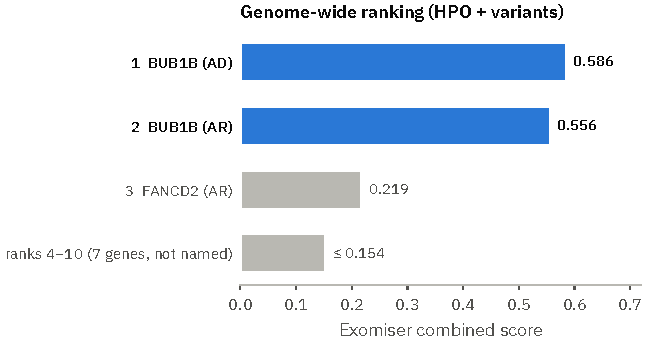
\includegraphics[width=\linewidth]{fig/t1_exomiser.pdf}\end{minipage}\hfill
\begin{minipage}[t]{0.47\linewidth}\vspace{0pt}{\sffamily\bfseries\small b}\\[6mm]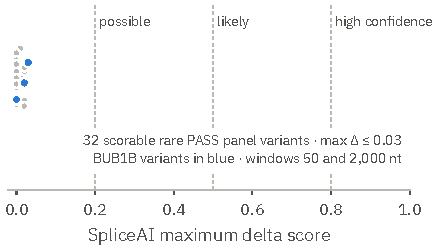
\includegraphics[width=\linewidth]{fig/t1_spliceai.pdf}\end{minipage}
\caption{\textbf{a}, Exomiser configuration A (configuration B gives the same top 3). Only the genes discussed in
the text are named; ranks 4–10 are shown only in aggregate. \textbf{b}, SpliceAI maximum delta for the 32 scorable rare PASS variants of the
MVA/SAC panel (\gene{BUB1B} variants in blue): none approaches the 0.2 threshold.}
\label{fig:fenotipo}
\end{figure}

\section{Candidate variants and ACMG/AMP classification}

Criteria follow \citet{richards} with ClinGen SVI refinements: the PVS1 decision tree \citep{pvs1}, PM2 downgraded
to Supporting, the PM3 point system for recessive disorders, and splicing guidance for BP4. Points follow
\citet{tavtigian}: Supporting 1, Moderate 2, Strong 4, Very strong 8, benign criteria negative; Pathogenic $\geq$ 10,
Likely pathogenic 6–9, VUS 0–5 (Figure~\ref{fig:acmg}).

\begin{figure}[htbp]
\centering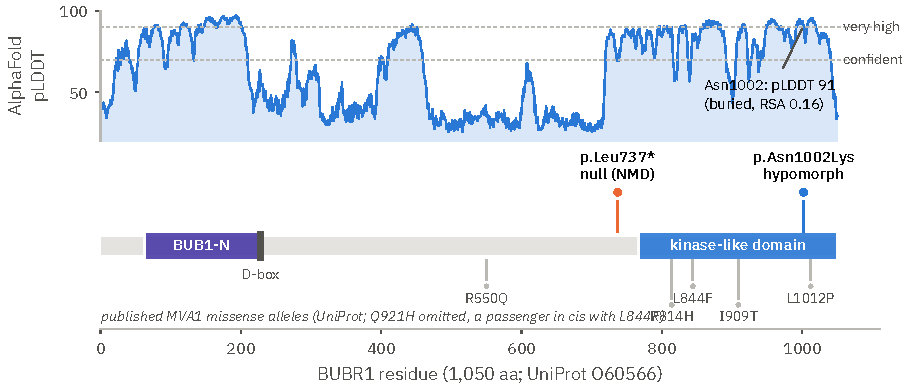
\includegraphics[width=\linewidth]{fig/t1_proteina.pdf}
\caption{Where the alleles fall on BUBR1. Top, AlphaFold confidence (pLDDT) of model AF-O60566-F1 v6. Bottom,
UniProt domains, the two alleles of this child (coloured) and the published MVA1 missense alleles (grey), 5 of 6 in
the kinase-like domain. Asn1002 is a high-confidence, largely buried residue (relative accessibility 0.16) packing
against residues 973–978 of the C-lobe, 12~Å from L1012. A longer, positively charged lysine there could
destabilise the fold, as the kinase-domain MVA1 missense alleles tested do \citep{suij}; the known stable-but-dysfunctional alleles lie
outside this domain, but this residue has never been characterised, so the class of this allele is unmeasured.}
\label{fig:proteina}
\end{figure}

\subsection{Allele 1 — c.2210T>G p.(Leu737*)}
The change converts the Leu codon TTA into a TGA (UGA) stop codon; BUBR1 is 1,050 amino acids long.

\begin{table}[H]\tablefont
\begin{tabularx}{\linewidth}{@{}P{2.75cm}LP{1.6cm}@{}}
\toprule\thead{Criterion} & \thead{Evidence} & \thead{Points}\\\midrule
PVS1 & Nonsense in exon 17 of 23: premature stop > 50 nt upstream of the last exon–exon junction, so NMD is predicted. Loss of function is the established mechanism of MVA1 (truncating alleles are degraded by NMD and yield no detectable protein; \citealp{suij}). Biologically relevant (MANE) transcript & +8\\
PM2\_Supporting & gnomAD v4.1 AF $7.9\times10^{-5}$ (exomes), $3.3\times10^{-5}$ (genomes), no homozygotes; compatible with a recessive disease & +1\\
PM3 & \emph{not applied.} The ClinGen SVI point system requires the \emph{trans} allele to be Pathogenic or Likely pathogenic; our partner allele is a VUS, and awarding PM3 here would make the two classifications bootstrap each other & 0\\
(ClinVar) & Pathogenic / Likely pathogenic, criteria provided, multiple submitters, no conflicts. Corroboration only; PP5 was retired by ClinGen SVI & —\\\midrule
\textbf{Total} & & \textbf{9 · Likely pathogenic}\\\bottomrule
\end{tabularx}\end{table}
Call quality: heterozygous, depth 46, allele fraction 0.54, GQ 99, PASS.

\subsection{Allele 2 — c.3006T>G p.(Asn1002Lys)}
\begin{table}[H]\tablefont
\begin{tabularx}{\linewidth}{@{}P{2.75cm}LP{1.8cm}@{}}
\toprule\thead{Criterion} & \thead{Evidence} & \thead{Points}\\\midrule
PM2\_Supporting & ultra-rare: absent from the VEP-annotated gnomAD v4.1 release; at most one allele in the gnomAD v4 exome NFE data used by Exomiser & +1\\
PP3 & AlphaMissense 0.923 \citep{alphamissense}, MVP 0.852, PolyPhen-2 0.997, SIFT 0.01; REVEL 0.472 is indeterminate, so PP3 is applied at Supporting only & +1\\
PM1\_Supporting & substitutions in or near the kinase-like domain (UniProt 766–1050) lower BUBR1 abundance 5–10$\times$, the documented disease mechanism \citep{suij}; 4 of the 5 MVA1 missense alleles annotated in UniProt sit there (Q921H is excluded: it is a functionally normal passenger in \emph{cis} with L844F); structural context in Figure~\ref{fig:proteina} & +1\\
PM3\_Supporting & with a pathogenic truncating allele in the same gene, phase unknown & +1\\
PP4 (contestable) & strictly PP4 asks for a \emph{single} genetic aetiology and MVA has $\geq$4 genes, so a reviewer may drop it; we apply it at Supporting because the cytogenetic phenotype plus rhabdomyosarcoma, a tumour recurrently reported in MVA1 & +1 (Moderate +2 defensible)\\
BP1 (proposed by Exomiser) & \textbf{not applied}: BP1 requires truncation to be the \textit{only} mechanism; hypomorphic missense alleles are an established MVA1 mechanism & 0\\\midrule
\textbf{Total} & & \textbf{4–5 · VUS} (upper end if PP4 is accepted)\\\bottomrule
\end{tabularx}\end{table}
This allele stays a VUS on points, and we say so rather than claim a borderline Likely pathogenic: dropping the
contestable PP4 leaves 4. Confirming \emph{trans} phase would raise PM3 to Moderate and, with PP4, reach Likely
pathogenic --- which is why parental testing is the single most valuable experiment here. Call quality: heterozygous, depth 28, allele fraction 0.46, GQ 99, PASS. SpliceAI delta 0.02.

\subsection{Alternative second allele — c.2679-1026A>G (deep intronic)}
Absent from gnomAD; allele fraction 0.39. SpliceAI delta 0.00 at both windows gives BP4 ($-1$); with PM2\_Supporting
(+1) the total is 0, a VUS that leans benign. It is kept in the CSV only as a low-probability hedge (EPCR 0.03 and
0.01).

\begin{figure}[htbp]
\centering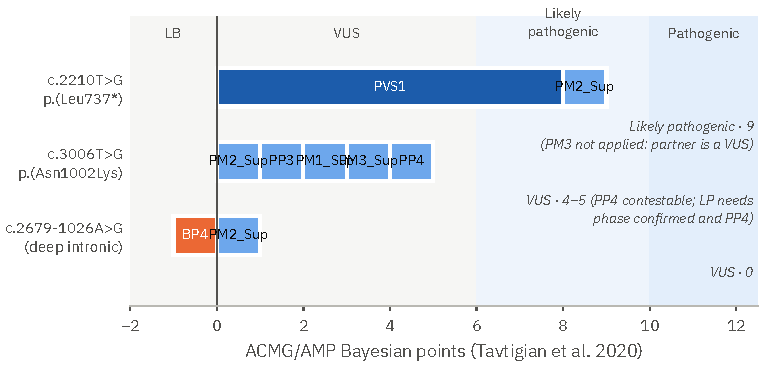
\includegraphics[width=0.8\linewidth]{fig/t1_acmg.pdf}
\caption{Bayesian ACMG/AMP points per submitted variant \citep{tavtigian}. Shaded bands are the class thresholds.}
\label{fig:acmg}
\end{figure}

\section{Phase}
\label{sec:phase}
The VCF carries no read-backed phase (\code{PGT/PID}) for these sites. The two alleles are 10,911~bp apart. With
PCR-free Illumina libraries no read or read pair can span them, and phasing through intermediate heterozygous sites
would need a chain of informative sites less than $\sim$500~bp apart. We tested this directly
(\code{fase\_viable.py}; Figure~\ref{fig:fase}). The interval contains only three PASS heterozygous sites, separated
by 6,769 and 4,142~bp, with no phase block, so no short-read chain can bridge them. Realigning the FASTQ ($\approx$1
USD targeted, 5–8 USD genome-wide) therefore cannot phase the pair, and was not done.

\begin{figure}[htbp]
\centering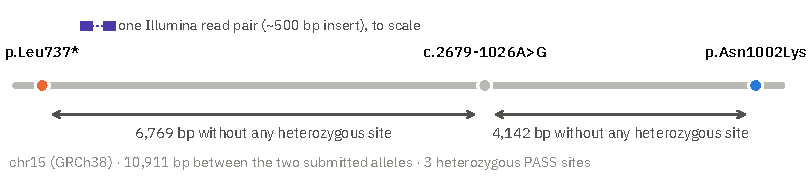
\includegraphics[width=\linewidth]{fig/t1_fase.pdf}
\caption{Why the pair cannot be phased from short reads: the only heterozygous sites in the interval are far apart
compared with one read pair, drawn to scale.}
\label{fig:fase}
\end{figure}

Phase is argued from evidence instead:
\begin{enumerate}
\item A \textit{cis} configuration would leave one fully wild-type \gene{BUB1B} copy. Monoallelic loss gives at most
  the milder premature chromatid separation trait \citep{matsuura}, never full MVA; BUBR1 function is dosage
  dependent, with aneuploidy appearing below $\sim$50\,\% residual protein \citep{bohers}.
\item The patient has a cytogenetic MVA diagnosis, and the genome has no other qualifying variant in any MVA/SAC
  gene, no second hit elsewhere in \gene{BUB1B}, and no alternative recessive diagnosis (§\ref{sec:alt}).
\item Both allele fractions are balanced (0.54 and 0.46). This is a quality control rather than a phase argument: it
  shows that both calls are genuine heterozygotes and excludes a large deletion of the other haplotype over either
  site; the 15q15 region is balanced as a whole (§\ref{sec:qc}).
\end{enumerate}
Trans is by far the most parsimonious configuration. Recommended clinical confirmation: targeted parental testing, or
long-read sequencing of the 11-kb interval.

\section{Genome-level checks: allelic balance, mosaicism and autozygosity}
\label{sec:qc}
Three checks computed in the protected environment (\code{balance\_alelico.py}). Only per-chromosome statistics
leave it.

\begin{figure}[htbp]
\centering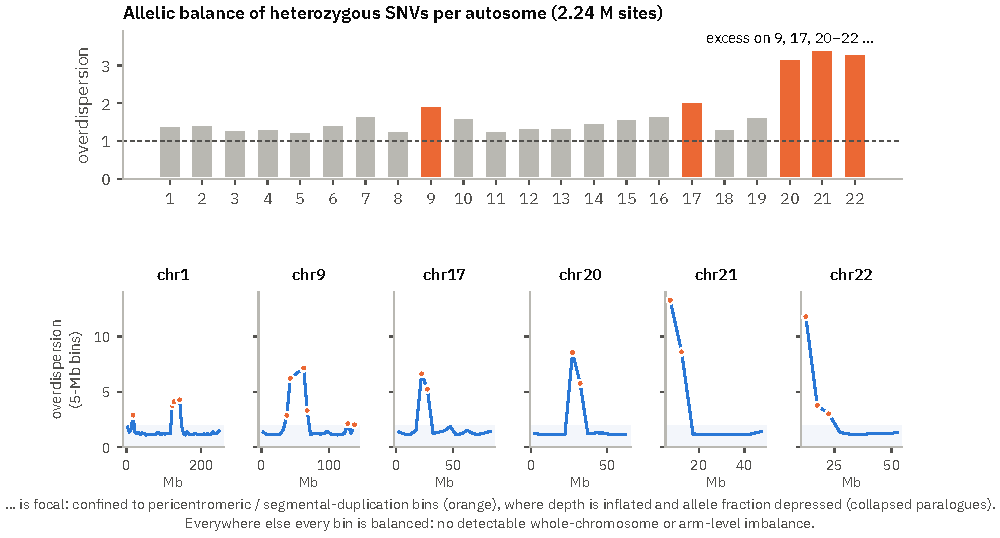
\includegraphics[width=\linewidth]{fig/t1_balance.pdf}
\caption{Allelic balance of 2.24\,M heterozygous SNVs (PASS, depth $\geq$ 20). Overdispersion is the observed variance
of allele fractions divided by the variance expected from binomial sampling at each site's depth; a mosaic gain or
loss would raise it along a whole chromosome or arm. Dashed line: binomial expectation (1).}
\label{fig:balance}
\end{figure}

\begin{enumerate}
\item \textbf{Allelic balance and mosaicism.} Per-chromosome overdispersion is 1.24–1.49 on most autosomes but
  higher on 9, 17 and 20–22. Binning at 5~Mb shows that \textbf{the excess is focal}: it is confined to
  pericentromeric and segmental-duplication regions, where depth is inflated (61–105$\times$ vs 44$\times$) and the
  allele fraction is depressed (0.30–0.40). That is the signature of collapsed paralogues, not of aneuploidy.
  Everywhere else every bin is balanced. No whole-chromosome or arm-level imbalance is detectable, which is expected in
  MVA: aneuploidy is \textit{variegated} (different chromosomes in different cells, each at a few percent) and
  cannot be resolved by bulk allele fractions. Karyotyping or single-cell methods remain the diagnostic standard.
\item \textbf{The \gene{BUB1B} locus.} \gene{BUB1B} ± 5~Mb: 6,312 heterozygous sites with median allele fraction
  0.50, so no loss of heterozygosity or imbalance around the gene. This supports both variants being genuine germline
  heterozygous calls.
\item \textbf{Autozygosity.} No run of homozygosity longer than 2~Mb in callable sequence. Runs were counted between
  consecutive heterozygous sites that still contain called homozygous-alternate sites, which excludes assembly gaps
  and centromeres; \code{bcftools roh} agrees. Extended autozygosity would have favoured a homozygous allele from
  consanguineous parents. Its absence fits the compound heterozygous model and the two different heterozygous
  alleles observed.
\end{enumerate}

\section{Mechanism: why this genotype explains the phenotype}
BUBR1 is a core component of the mitotic checkpoint complex, which inhibits APC/C–CDC20 until every kinetochore is
attached; it also stabilises kinetochore–microtubule attachments. Cells from patients with biallelic \gene{BUB1B}
mutations show an impaired checkpoint, misaligned chromosomes and low total BUBR1 \citep{suij}. The truncating
allele is removed by NMD, and the kinase-domain missense proteins tested are rapidly degraded; the known
stable-but-dysfunctional alleles lie outside this domain. The residual BUBR1 is enough
for viability but not for faithful segregation, hence mosaic aneuploidies in many tissues.

\begin{table}[H]\tablefont
\begin{tabularx}{\linewidth}{@{}P{3.6cm}L@{}}
\toprule\thead{Phenotype (HPO)} & \thead{Fit with biallelic \gene{BUB1B}}\\\midrule
Rhabdomyosarcoma & recurrently reported in MVA1 \citep{hanks,nishitani}; MVA is on the AACR list of childhood genomic-instability cancer predisposition syndromes \citep{nakano}\\
Growth failure, short stature, SGA & core MVA features\\
Skeletal muscle atrophy & early sarcopenia in BubR1-hypomorphic mice \citep{baker04}; sarcopenia correlated with mTORC1 hyperactivity in mice carrying a single MVA allele; the biallelic genotype closest to this child (X753/L1002P) died prematurely \citep{sieben}\\
Recurrent spontaneous abortion (family) & not explained by this genotype, which is viable in the child; not diagnostic\\
Nephrocalcinosis & not a classical MVA feature; left unexplained (possibly treatment- or prematurity-related; no nephrocalcinosis-gene variant passed the funnel)\\\bottomrule
\end{tabularx}\end{table}

\section{Alternative hypotheses excluded}
\label{sec:alt}
{\tablefont
\begin{xltabular}{\linewidth}{@{}P{4.2cm}P{3.9cm}L@{}}
\toprule\thead{Hypothesis} & \thead{What was checked} & \thead{Result}\\\midrule\endhead
\midrule\multicolumn{3}{r}{\textcolor{muted}{continued on next page}}\\\endfoot\bottomrule\endlastfoot
Other MVA genes (\gene{CEP57, TRIP13, CENATAC}) and the SAC panel & every consequence, AF < 5\,\%, SpliceAI & no rare qualifying or splice-altering variant\\
Other recessive diagnoses & the 98 non-panel genes of the funnel, one by one & hypervariable or paralogous regions (HLA, KIR, MUC, KRTAP, ZNF, olfactory/taste receptors, pseudogenes), ClinVar-benign variants, low-depth homozygous artefacts (2–6 reads), or no phenotype fit\\
Exomiser rank 3 (\gene{FANCD2}) & variant-level review & two adjacent deletions on a non-canonical transcript, ClinVar benign: artefact\\
Dominant rhabdomyosarcoma predisposition & \gene{TP53, DICER1, NF1}; RASopathy genes; Beckwith–Wiedemann (\gene{CDKN1C}, H19/IGF2); \gene{SMARCB1}; Lynch; \gene{PTCH1/SUFU} & no rare functional variant\\
Other chromosome-instability syndromes (Bloom, Werner, Rothmund–Thomson, Roberts/\gene{ESCO2}, Fanconi) & coding + splice & no biallelic qualifying variant\\
Mulibrey nanism (\gene{TRIM37}), recently reported with MVA (\pmid{41702694}) & coding + splice + Exomiser & no rare functional variant; Exomiser score 0\\
Mosaic aneuploidy detectable in bulk data & allelic balance, 5-Mb bins & none beyond artefact regions (§\ref{sec:qc})\\
Incidental findings & genome-wide & handled per the organisers' IRB guidance; not reported\\
\end{xltabular}}

\section{Ranking strategy and EPCR}
\begin{table}[H]\tablefont
\begin{tabularx}{\linewidth}{@{}P{0.5cm}P{4.3cm}P{1.0cm}L@{}}
\toprule\thead{Row} & \thead{Variants} & \thead{EPCR} & \thead{Rationale}\\\midrule
1 & c.2210T>G + c.3006T>G & 0.95 & pathogenic null + hypomorph in the only gene supported by genotype and phenotype; Exomiser \#1\\
2 & c.2210T>G + c.2679-1026A>G & 0.03 & the only other rare \gene{BUB1B} variant; SpliceAI 0.00, so very unlikely\\
3 & c.3006T>G + c.2679-1026A>G & 0.01 & excludes the only pathogenic allele: least likely\\\bottomrule
\end{tabularx}\end{table}
EPCR values are a calibrated judgement. The residual 1–5\,\% covers phase uncertainty and the unobservable
possibility of a structural or deep regulatory allele missed by short-read calls. The two hedge rows cost nothing
if row 1 is correct, because F-max is taken at the best threshold. No secondary findings are submitted. The file was
validated with the organisers' \code{evaluation.py}.

\section{Limitations}
\begin{itemize}
\item No BAM/CRAM: structural variants, copy-number changes and repeat expansions were not called genome-wide; the
  balanced allele fractions only exclude deletions spanning the two sites.
\item Phase is inferred, not observed (§\ref{sec:phase}).
\item The VEP and Exomiser gnomAD snapshots differ slightly for allele 2 (absent vs one allele); both support PM2.
\item Predictors disagree in magnitude for allele 2 (REVEL intermediate, AlphaMissense high), so PP3 was applied at
  Supporting only.
\item Single proband: no segregation evidence (PP1).
\end{itemize}

\section{Reproducibility}
All scripts are in the repository; each Modal run is logged with its cost in \code{scripts/modal/gastos.csv}.
Pinned versions: VEP 116 (cache 116, GRCh38), gnomAD v4.1, AlphaMissense hg38, ClinVar NCBI (October 2026), Exomiser
15.1.0 with data 2512, SpliceAI 1.3.1 (TensorFlow 2.15). Figures are regenerated by \code{scripts/figuras/figuras\_t1.py}
and this document by \code{scripts/compila\_informes.py}.
\begin{keybox}
\ttfamily\footnotesize
python scripts/hpo\_extraer.py\hfill\# HPO IDs (labels: local hp.obo)\\
python scripts/modal/refs.py \&\& python scripts/modal/exomiser\_refs.py\hfill\# public references\\
python scripts/modal/anotar.py --subir \&\& python scripts/modal/filtra.py\hfill\# annotate, funnel, panel\\
python scripts/modal/splice\_ai.py \&\& python scripts/modal/exomiser.py\hfill\# splicing, phenotype\\
python scripts/modal/fase\_viable.py\hfill\# phasability test\\
python scripts/modal/balance\_alelico.py [--diagnostico|--roh]\hfill\# genome-level QC
\end{keybox}

\section{Data protection and LLM use}
\label{sec:data}
\begin{itemize}
\item \textbf{LLM declaration} (organisers' format, discussion \#2, 28 September 2026): \textit{Anthropic Claude via the
  Claude Code CLI, Claude Max (consumer tier), model-training opt-out enabled (``Help improve Claude'' off), no
  feedback provided on any output, no content flagged for safety review.}
\item \textbf{Applicable data-handling terms} (discussion \#21): opted-out conversations are not used for training and
  are retained for 30 days. The two exceptions (feedback, safety flags) were avoided, and feedback, bug-report and
  transcript-sharing commands were disabled by configuration.
\item \textbf{Data minimisation}, as an added precaution: the model saw code, aggregate counts, HPO terms and short
  candidate lists ($\leq$ 50 annotated variants). The raw data and genome-scale derivatives in \code{data/} were blocked
  from the agent by configuration; intermediate tables were processed only by scripts, never loaded whole into the
  model context (\code{docs/llm\_use.md}).
\item \textbf{Compute:} Modal (data processor, no training on customer data). The case VCF lives in a private volume
  that will be deleted within 30 days of the close. No patient variant was sent to any third-party API; all
  annotation used downloaded public resources.
\item \textbf{Incidental findings:} handled as advised by the organisers in discussion \#20. They are not named in any
  public material, the family and clinical team are not contacted, and the organisers have escalated the question
  to the study IRB.
\end{itemize}

\section*{Acknowledgement}
This work was made possible through the Hackathon, organized by Sage Bionetworks in partnership with the MVA Society,
Hugging Face, and BEACON (The Benchmarking, Evaluation, and Assessment Consortium for Science), with prize sponsorship
from AWS and Anthropic. We are deeply grateful to the child and their family who generously contributed their data
and their story to advance research into this rare disease. We acknowledge their trust in making this Hackathon
possible.

{\small Dataset: SageBio. \textit{Rare Disease, Real Kid: MVA Hackathon 2026 — Dataset}. Hugging Face,
\code{SageBio/mva-hackathon-2026-data}, 2026.}

\section*{References}
\begin{refs}
\item Abou Tayoun AN et al. Recommendations for interpreting the loss of function PVS1 ACMG/AMP variant criterion. \textit{Hum Mutat} 2018. \pmid{30192042}.
\item Baker DJ et al. BubR1 insufficiency causes early onset of aging-associated phenotypes and infertility in mice. \textit{Nat Genet} 2004. \pmid{15208629}.
\item Bohers E et al. Gradual reduction of BUBR1 protein levels results in premature sister-chromatid separation then in aneuploidy. \textit{Hum Genet} 2008. \pmid{18932004}.
\item Cheng J et al. Accurate proteome-wide missense variant effect prediction with AlphaMissense. \textit{Science} 2023. \pmid{37733863}.
\item Hanks S et al. Constitutional aneuploidy and cancer predisposition caused by biallelic mutations in BUB1B. \textit{Nat Genet} 2004. \pmid{15475955}.
\item Jaganathan K et al. Predicting splicing from primary sequence with deep learning. \textit{Cell} 2019. \pmid{30661751}.
\item Malumbres M. Mosaic variegated aneuploidy in development, ageing and cancer. \textit{Nat Rev Genet} 2024. \pmid{39169218}.
\item Matsuura S et al. Monoallelic BUB1B mutations and defective mitotic-spindle checkpoint in seven families with premature chromatid separation syndrome. \textit{Am J Med Genet A} 2006. \pmid{16411201}.
\item Nakano Y et al. Update on recommendations for cancer screening and surveillance in children with genomic instability disorders. \textit{Clin Cancer Res} 2024. \pmid{39264246}.
\item Nishitani-Isa M et al. Rhabdomyosarcoma with premature chromatid separation–mosaic variegated aneuploidy syndrome: reduced-intensity chemotherapy. \textit{Pediatr Int} 2019. \pmid{31184400}.
\item Richards S et al. Standards and guidelines for the interpretation of sequence variants. \textit{Genet Med} 2015. \pmid{25741868}.
\item Sieben CJ et al. BubR1 allelic effects drive phenotypic heterogeneity in mosaic-variegated aneuploidy progeria syndrome. \textit{J Clin Invest} 2020. \pmid{31738183}.
\item Smedley D et al. Next-generation diagnostics and disease-gene discovery with the Exomiser. \textit{Nat Protoc} 2015. \pmid{26562621}.
\item Snape K et al. Mutations in CEP57 cause mosaic variegated aneuploidy syndrome. \textit{Nat Genet} 2011. \pmid{21552266}.
\item Suijkerbuijk SJ et al. Molecular causes for BUBR1 dysfunction in the human cancer predisposition syndrome mosaic variegated aneuploidy. \textit{Cancer Res} 2010. \pmid{20516114}.
\item Tavtigian SV et al. Fitting a naturally scaled point system to the ACMG/AMP variant classification guidelines. \textit{Hum Mutat} 2020. \pmid{32720330}.
\item Yost S et al. Biallelic TRIP13 mutations predispose to Wilms tumor and chromosome missegregation. \textit{Nat Genet} 2017. \pmid{28553959}.
\item Hakonen AH et al. Mosaic variegated aneuploidy as a novel feature in patients with Mulibrey nanism and TRIM37 variants. \textit{J Med Genet} 2026. \pmid{41702694}.
\end{refs}

\clearpage
\appendix
\section{Methods description form (Track 1 methods)}
\textit{Answers to the organisers' official methods description template (version with the required LLM question), reproduced here because the submission form has no separate upload field for it.}

\begin{description}[leftmargin=0pt,style=nextline,itemsep=4pt,font=\sffamily\bfseries\small\color{branddark}]
\item[Team name] aperezcastro (Agustín Pérez Castro, individual)
\item[Model number (fill out this form once per model/approach submitted; up to 6)] 1 (BUB1B compound heterozygous; aperezcastro\_bub1b\_comphet.csv)
\item[Please describe your model/approach in detail.] Three-arm pipeline on the provided VCF, run as time-capped jobs on Modal (scripts in the GitHub repo). (1) bcftools norm (split multiallelics, left-align vs Ensembl GRCh38) $\rightarrow$ Ensembl VEP 116 offline (MANE, HGVS, gnomAD v4.1 exomes+genomes, ClinVar with review status, SIFT, PolyPhen-2, AlphaMissense). (2) Unbiased genome-wide funnel: PASS $\rightarrow$ max gnomAD AF < 1\% $\rightarrow$ HIGH/MODERATE/splice $\rightarrow$ gene-level recessive model ($\geq$2 het or 1 hom) = 339 variants in 99 genes, each reviewed. (3) Hypothesis-driven arm: MVA/spindle-assembly-checkpoint panel (BUB1B, CEP57, TRIP13, CENATAC, BUB1, BUB3, MAD1L1, MAD2L1BP, SMC5/6 complex...) at any consequence and AF < 5\%; of the 42 rare PASS variants, the 32 inside annotated gene bodies were scored with SpliceAI 1.3.1 (50 and 2000 nt windows; all max delta $\leq$ 0.03). (4) Exomiser 15.1 (data 2512) with the 8 HPO terms, with and without a phenotype pre-filter: BUB1B ranks \#1 genome-wide in both. (5) ACMG/AMP classification with ClinGen SVI refinements and Bayesian points (Tavtigian 2020) for each submitted variant; phase feasibility tested directly (only 3 heterozygous sites in the 10.9 kb interval, gaps 6.8 and 4.1 kb: not phasable with short reads) and argued from biology. (6) Genome-level QC from aggregate statistics: allelic balance per autosome and in 5-Mb bins (excess overdispersion confined to pericentromeric/segmental-duplication regions, i.e. technical; no detectable whole-chromosome imbalance, as expected for variegated low-level mosaicism), balanced allele fractions around BUB1B, and no run of homozygosity > 2 Mb (consistent with compound heterozygosity rather than autozygosity). Answer: BUB1B c.2210T>G p.(Leu737*) [Likely pathogenic, 9 points; Pathogenic with ClinVar corroboration] + c.3006T>G p.(Asn1002Lys) [VUS, 4-5 points], MVA type 1.
\item[(required) If commercially-available Generative AI was used, record the provider, the plan or tier, and the relevant setting in your methods description. A line is enough, for example, "Anthropic API, Claude Sonnet, commercial terms, no training on customer content."] Anthropic Claude via the Claude Code CLI (Claude Opus models), Claude Max (consumer tier), model-training opt-out enabled ('Help improve Claude' off), no feedback provided on any output, no content flagged for safety review - per the organisers' confirmed guidance of 28 Sep 2026 (discussion \#2). Applicable terms: opted-out conversations are not used for training and are retained 30 days. Additional data minimisation: the model only saw code, aggregate counts, HPO terms and short candidate lists ($\leq$ 50 annotated variants); raw data and genome-scale derivatives were blocked from the agent by configuration. No patient variant was sent to any third-party API.
\item[Please state whether the submission file is the automated output of your computational approach (preferred), or if it has undergone downstream manual review and curation.] Candidate generation is automated (funnel, panel, SpliceAI, Exomiser); the final 3-row file and EPCR values were curated manually from the automated evidence.
\item[Please describe any downstream manual review in detail.] Manual review of the 99 recessive candidate genes (artefact-prone regions, ClinVar-benign, low depth, phenotype fit), of Exomiser's top hits, and of dominant rhabdomyosarcoma predisposition genes. Row 1 = the pair (EPCR 0.95). Rows 2-3 are low-probability alternative pairings with a third rare deep-intronic BUB1B variant (SpliceAI 0.00; EPCR 0.03 and 0.01). EPCR reflects residual uncertainty about phase and unobserved SV/regulatory alleles. Validated with the organisers' evaluation.py.
\item[Please state whether your approach only used publicly available data (preferred) or if proprietary data was also used. If proprietary data were used, where possible, please also include a submission based only on publicly available data.] Only publicly available data.
\item[Please describe any public data used in detail (e.g., reference panels, population databases, literature).] GRCh38 (Ensembl 116 primary assembly), Ensembl VEP 116 cache, GENCODE (SpliceAI grch38), gnomAD v4.1, ClinVar (NCBI VCF, Oct 2026), AlphaMissense hg38, Exomiser data release 2512 (REVEL, MVP, AlphaMissense, SpliceAI, HPO/MGI/ZFIN phenotypes), Human Phenotype Ontology (hp.obo), UniProt O60566 and the AlphaFold model, PubMed literature (cited in the report).
\item[Please describe any proprietary data used in detail.] None.
\item[Is your approach able to output proposed pairs of compound heterozygous candidate variants, or only single candidate variants?] Yes: pairs are produced by the gene-level recessive model (all qualifying pairs within a gene) and ranked; single variants are produced for dominant models.
\item[How did you handle secondary or incidental findings, if any? (See the finding\_type column in your submission.)] No secondary findings were submitted. Incidental findings were handled following the organisers' IRB guidance (discussion \#20) and are not reported.
\item[Please provide an estimate of run time and cost for your approach (if possible).] About 1 hour wall-clock of cloud compute (annotation parallelised over 25 containers \textasciitilde{}20 min, Exomiser \textasciitilde{}7 min, SpliceAI \textasciitilde{}4 min) plus reference downloads; total Modal cost \textasciitilde{}1.4 USD (scripts/modal/gastos.csv). Reproducible from the repository.
\item[Provide a method abstract (up to 500 words). Please include strengths and limitations of your method as well as methodological detail.] We combined an unbiased genome-wide search with a hypothesis-driven analysis of genes linked to mosaic variegated aneuploidy (MVA). The single-sample WGS VCF was normalised and annotated offline with Ensembl VEP 116 (gnomAD v4.1, ClinVar, AlphaMissense) on a private cloud environment. A recessive gene-level funnel reduced 4.96 M variants to 339 variants in 99 genes, of which only BUB1B belongs to the MVA/spindle-checkpoint panel. Because the second, hypomorphic allele in MVA1 is often subtle, the panel was searched at every consequence class and scored with SpliceAI; independently, Exomiser 15.1 with the patient's HPO terms ranked BUB1B first genome-wide with and without a phenotype filter (score 0.59 dominant / 0.56 recessive vs $\leq$ 0.22 for the next gene). The proband carries BUB1B c.2210T>G p.(Leu737*) (nonsense, NMD predicted; ClinVar P/LP; ACMG 9 points, Likely pathogenic, Pathogenic with ClinVar corroboration) and c.3006T>G p.(Asn1002Lys) (ultra-rare kinase-domain missense, AlphaMissense 0.92, buried high-confidence residue in the AlphaFold model 12 Å from the known MVA1 allele L1012P; 4-5 points, VUS; its class, low abundance or impaired function, is unmeasured). This null + kinase-domain hypomorph architecture is the classical MVA1 pattern and mirrors a published mouse model (BubR1 X753 + L1002P, mouse L1002 = human L1012). A third rare deep-intronic BUB1B variant was assessed and deprioritised (SpliceAI 0.00). Phase could not be observed: the 10.9 kb interval contains only three heterozygous sites (gaps 6.8 and 4.1 kb), so we tested and documented that short-read phasing is infeasible and argued trans configuration from biology (monoallelic loss does not cause MVA), absence of any other qualifying variant and balanced allele fractions, and the genome shows no run of homozygosity > 2 Mb. Strengths: three independent arms converging on the same pair, explicit ACMG evidence with Bayesian points, sensitivity to subtle alleles, full reproducibility with cost-capped scripts, and strict data minimisation (no third-party variant APIs). Limitations: no BAM/CRAM, so structural variants were not called genome-wide; phase is inferred rather than observed; in silico predictors disagree in magnitude for the missense (REVEL 0.47); single proband without segregation data.
\end{description}


\end{document}
